%% Committee Presentation — Climate Shocks & Health Finance
%% Formatted following MixtapeTools/presentations conventions
\documentclass[aspectratio=169,11pt]{beamer}

% ── Packages ──────────────────────────────────────────────────────────────────
\usepackage{graphicx}
\usepackage{booktabs}
\usepackage{array}
\usepackage{xcolor}
\usepackage{tikz}
\usetikzlibrary{calc, positioning}
\usepackage{amsmath}
\usepackage{siunitx}
\usepackage{hyperref}

% ── Colour Palette ────────────────────────────────────────────────────────────
\definecolor{DeepNavy}{HTML}{2E4057}
\definecolor{Teal}{HTML}{048A81}
\definecolor{WarmOrange}{HTML}{E85D04}
\definecolor{SoftPurple}{HTML}{9D4EDD}
\definecolor{WarmGray}{HTML}{8A8A8A}
\definecolor{LightGray}{HTML}{F2F2F2}
\definecolor{Cream}{HTML}{FFFDF7}
\definecolor{DeepRed}{HTML}{C1121F}
\definecolor{Gold}{HTML}{D4A017}

% ── Theme Setup ───────────────────────────────────────────────────────────────
\usetheme{default}
\setbeamertemplate{navigation symbols}{}
\setbeamertemplate{headline}{}

% Background
\setbeamercolor{background canvas}{bg=Cream}

% Frame title
\setbeamercolor{frametitle}{fg=DeepNavy,bg=Cream}
\setbeamerfont{frametitle}{series=\bfseries,size=\Large}
\setbeamertemplate{frametitle}{%
  \vspace*{0.4em}%
  \hspace*{0.3cm}\insertframetitle%
  \ifx\insertframesubtitle\empty\else
    \\[0.1em]\hspace*{0.3cm}{\footnotesize\color{WarmGray}\insertframesubtitle}%
  \fi
  \par\vspace*{0.15em}%
  \textcolor{Teal}{\rule{\textwidth}{0.5pt}}%
}

% Footline — page numbers only
\setbeamertemplate{footline}{%
  \hfill{\color{WarmGray}\tiny\insertframenumber\hspace{0.5em}}%
  \vspace{0.3em}%
}

% Bullets
\setbeamercolor{itemize item}{fg=Teal}
\setbeamercolor{itemize subitem}{fg=WarmOrange}
\setbeamertemplate{itemize item}{\small\raisebox{0.15ex}{\textbullet}}
\setbeamertemplate{itemize subitem}{\scriptsize\raisebox{0.15ex}{\textbullet}}

% Block colours
\setbeamercolor{block title}{fg=white,bg=DeepNavy}
\setbeamercolor{block body}{fg=DeepNavy,bg=LightGray}
\setbeamercolor{block title alerted}{fg=white,bg=WarmOrange}
\setbeamercolor{block body alerted}{fg=DeepNavy,bg=LightGray}
\setbeamercolor{block title example}{fg=white,bg=Teal}
\setbeamercolor{block body example}{fg=DeepNavy,bg=LightGray}

% ── Custom Macros ─────────────────────────────────────────────────────────────
\newcommand{\emphcolor}[1]{{\color{WarmOrange}\textbf{#1}}}
\newcommand{\tealtext}[1]{{\color{Teal}#1}}
\newcommand{\navytext}[1]{{\color{DeepNavy}#1}}
\newcommand{\graytext}[1]{{\color{WarmGray}#1}}

\newcommand{\transitionslide}[2]{%
  \begingroup
  \setbeamercolor{background canvas}{bg=DeepNavy}
  \setbeamertemplate{footline}{}
  \begin{frame}[plain]
    
\begin{tikzpicture}[overlay]
      % Teal accent triangle — coords relative to lower-left of text area
      \draw[Teal, opacity=0.3, line width=8pt]
        (-1,-1) -- ++(20,0) -- ++(0,12) -- cycle;
    \end{tikzpicture}
    \vspace{1.8cm}
    \hspace{0.8cm}%
    {\color{white}\bfseries\LARGE\parbox{13cm}{#1}}\\[0.6em]
    \hspace{0.8cm}%
    {\color{Teal}\normalsize\parbox{13cm}{#2}}
  \end{frame}%
  \endgroup
}

% ══════════════════════════════════════════════════════════════════════════════
\begin{document}

% ── Title frame ───────────────────────────────────────────────────────────────
\begingroup
\setbeamercolor{background canvas}{bg=DeepNavy}
\setbeamertemplate{footline}{}
\begin{frame}[plain]
  % Watermark
  \begin{tikzpicture}[overlay]
    \node[text=Teal, opacity=0.12, font=\fontsize{140}{140}\selectfont]
      at (10, 2.5) {\(\sim\)};
  \end{tikzpicture}
  \vspace{0.5cm}
  \hspace{0.6cm}%
  {\color{white}\bfseries\fontsize{22}{28}\selectfont
    \parbox{13cm}{Climate Shocks, Health Finance,\\and Economic Outcomes}}
  \par\vspace{0.5em}
  \hspace{0.6cm}%
  {\color{WarmOrange}\rule{12cm}{2pt}}
  \par\vspace{0.5em}
  \hspace{0.6cm}%
  {\color{Teal}\normalsize County-Level Evidence from the United States, 2011--2023}
  \par\vspace{0.4em}
  \hspace{0.6cm}%
  {\color{WarmGray}\small Thesis Committee Update \(\cdot\) March 2026}
\end{frame}
\endgroup

% ── TLDR ──────────────────────────────────────────────────────────────────────
\begin{frame}{Bottom Line Up Front}
  \begin{columns}[T]
    \begin{column}{0.48\textwidth}
      \begin{block}{\textbf{What we find}}
        \small\begin{itemize}\itemsep0.3em
          \item \emphcolor{Extreme cold} raises premiums \emphcolor{+\$31/yr} (7\%) and bad debt \emphcolor{+\$4.43/capita}; effects dissipate within 2--3 years
          \item \emphcolor{Extreme heat} leaves health costs unchanged but cuts household income \emphcolor{--\$265/yr}
          \item Drought \& AQI: \navytext{suggestive, not yet causally identified}
        \end{itemize}
      \end{block}
    \end{column}
    \begin{column}{0.48\textwidth}
      \begin{exampleblock}{\textbf{Why it matters}}
        \small\begin{itemize}\itemsep0.3em
          \item \tealtext{Two distinct pathways}: cold hits health-cost system; heat hits income
          \item Robust across DL (Distributed Lags) and LP (Local Projections) estimators; parallel trends hold for cold \& heat
          \item 3,225 counties $\times$ 2011--2023; county + year FE; state-clustered SEs
        \end{itemize}
      \end{exampleblock}
      \vspace{0.25em}
      \begin{alertblock}{\textbf{Novel contribution}}
        \small First county-level causal evidence linking climate shocks to \emphcolor{health finance outcomes}
      \end{alertblock}
    \end{column}
  \end{columns}
\end{frame}

% ── Roadmap ───────────────────────────────────────────────────────────────────
\begin{frame}{Today's Overview}
  \begin{columns}[T]
    \begin{column}{0.48\textwidth}
      \begin{enumerate}\itemsep0.5em
        \item \tealtext{Motivation \& Research Questions}
        \item \tealtext{Data \& Sample}
        \item \tealtext{Methodology}
        \item \emphcolor{Main Results: Cold Story}
        \item \emphcolor{The Heat Paradox}
        \item \navytext{Drought \& Air Quality}
        \item \navytext{Robustness}
        \item \navytext{Policy Implications}
      \end{enumerate}
    \end{column}
    \begin{column}{0.48\textwidth}
      \begin{block}{Status}
        \begin{itemize}
          \item State-level analysis: \tealtext{complete}
          \item County-level: \tealtext{complete}
          \item Event study: \tealtext{complete}
          \item Writing: in progress
        \end{itemize}
      \end{block}
    \end{column}
  \end{columns}
\end{frame}

% ══════════════════════════════════════════════════════════════════════════════
\transitionslide{Motivation \& Research Questions}{Why should climate shocks affect health costs?}

% ── Motivation ────────────────────────────────────────────────────────────────
\begin{frame}{Climate Shocks Create Financial Exposure}
  \begin{columns}[T]
    \begin{column}{0.56\textwidth}
      \textbf{The chain of transmission:}
      \begin{enumerate}\itemsep0.2em
        \item Climate event (cold snap, drought, bad air)
        \item Acute health utilisation spike
        \item Insurers absorb costs \(\rightarrow\) raise premiums
        \item Uninsured/underinsured face bad debt
        \item Household financial distress \(\rightarrow\) medical debt
      \end{enumerate}
      \vspace{0.3em}
      \textbf{This paper asks:}
      \begin{itemize}\itemsep0.2em
        \item Which shocks matter? \tealtext{Cold, heat, drought, or AQI?}
        \item What is the timing? \tealtext{Immediate or multi-year?}
        \item Is there an income channel? \tealtext{Separate from health costs?}
      \end{itemize}
    \end{column}
    \begin{column}{0.40\textwidth}
      \begin{alertblock}{State-Level Finding (prior work)}
        Extreme Drought (2-yr lag) and Cold Shocks (1-yr lag) \emphcolor{increase} Medical Debt and Insurance Premiums at the state level.\\[0.5em]
        \graytext{\small Now testing county-level with richer variation.}
      \end{alertblock}
    \end{column}
  \end{columns}
\end{frame}

% ── Gap in Literature ─────────────────────────────────────────────────────────
\begin{frame}{Literature Gap: Finance Channel Under-studied}
  \begin{columns}[T]
    \begin{column}{0.31\textwidth}
      \begin{exampleblock}{Environmental\\Science}
        Climate–health\\ exposure links\\[0.3em]
        {\footnotesize Gasparrini et al.\\ Carleton et al.\\ Burke et al.}
      \end{exampleblock}
    \end{column}
    \begin{column}{0.31\textwidth}
      \begin{exampleblock}{Health\\Economics}
        Insurance\\ market design\\[0.3em]
        {\footnotesize Gruber (2011)\\ Finkelstein (2007)\\ Handel et al.}
      \end{exampleblock}
    \end{column}
    \begin{column}{0.31\textwidth}
      \begin{alertblock}{\textbf{This Paper}}
        \emphcolor{Climate shocks}\\ $\rightarrow$ \emphcolor{health finance}\\ outcomes\\[0.3em]
        {\footnotesize County panel,\\ dynamic lags,\\ causal inference}
      \end{alertblock}
    \end{column}
  \end{columns}
  \vspace{0.8em}
  \begin{center}
    \tealtext{Bridges environmental science and health economics\\
    via a credible county-level identification strategy}
  \end{center}
\end{frame}

% ══════════════════════════════════════════════════════════════════════════════
\transitionslide{Data \& Sample}{3,225 counties $\times$ 13 years (2011--2023)}

% ── Data Sources ──────────────────────────────────────────────────────────────
\begin{frame}{Data Sources}
  \begin{columns}[T]
    \begin{column}{0.48\textwidth}
      \textbf{Climate / Environment}
      \begin{itemize}
        \item \tealtext{NOAA NCEI:} county CDD, HDD, temp, precip
        \item \tealtext{NOAA:} PDSI drought index (state)
        \item \tealtext{EPA:} Annual AQI by county monitor
      \end{itemize}
      \vspace{0.5em}
      \textbf{Health Finance}
      \begin{itemize}
        \item \tealtext{HIX Compare:} ACA benchmark premiums
        \item \tealtext{Urban Institute:} County medical debt
        \item \tealtext{NASHP:} Hospital bad debt / charity
      \end{itemize}
    \end{column}
    \begin{column}{0.48\textwidth}
      \textbf{Economic Controls}
      \begin{itemize}
        \item \tealtext{BEA CAINC1:} Per capita personal income
        \item \tealtext{ACS B19013:} Median household income
        \item \tealtext{ACS B23025:} Civilian employment
        \item \tealtext{FRED:} CPI for real-dollar conversion
      \end{itemize}
      \vspace{0.5em}
      \begin{block}{Panel Dimensions}
        \small 3,225 counties, 2011--2023\\
        41,376 county-year observations\\
        53 variables in master file
      \end{block}
    \end{column}
  \end{columns}
\end{frame}

% ── Descriptive Stats ─────────────────────────────────────────────────────────
\begin{frame}{Premiums Rising; Debt Prevalence Falling}
  \begin{center}
    \small
    \begin{tabular}{lrrrc}
      \toprule
      \textbf{Outcome} & \textbf{2011--16} & \textbf{2017--23} & \textbf{Change} & \textbf{\%} \\
      \midrule
      Benchmark Silver Premium (2023 USD) & \$287 & \$411 & +\$124 & \emphcolor{+43\%} \\
      Medical Debt Share (\%)             & 21.8  & 16.1  & --5.8 pp & \tealtext{--27\%} \\
      Uninsured Rate (\%)                 & 14.1  & 9.9   & --4.2 pp & \tealtext{--30\%} \\
      Median HH Income (2023 USD)         & \$60,499 & \$64,441 & +\$3,942 & +6.5\% \\
      \bottomrule
    \end{tabular}
  \end{center}
  \vspace{0.5em}
  \begin{columns}[T]
    \begin{column}{0.48\textwidth}
      \begin{alertblock}{Premiums surge}
        ACA market maturation + risk-pool age shift + subsidy design
      \end{alertblock}
    \end{column}
    \begin{column}{0.48\textwidth}
      \begin{exampleblock}{Debt prevalence falls}
        Coverage expansion + real income growth offset acute shocks
      \end{exampleblock}
    \end{column}
  \end{columns}
\end{frame}

% ── Shock Definitions ─────────────────────────────────────────────────────────
\begin{frame}{Climate Shock Definitions}
  \begin{columns}[T]
    \begin{column}{0.54\textwidth}
      \small
      \begin{tabular}{lll}
        \toprule
        \textbf{Shock} & \textbf{Definition} & \textbf{Prev.} \\
        \midrule
        \texttt{High\_CDD} & CDD $\geq$ 1,902 (p80) & 24\% \\
        \texttt{High\_HDD} & HDD $\geq$ 5,752 (p80) & 17\% \\
        \texttt{Is\_Extreme\_Drought} & PDSI $\leq -4$ & 2.3\% \\
        \texttt{High\_AQI\_Max} & Max AQI $> 100$ & 9.2\% \\
        \bottomrule
      \end{tabular}
      \vspace{0.5em}\\
      \textbf{Design choice:} National p80 thresholds from 1990--2000 baseline\\[0.2em]
      \graytext{\footnotesize ``Physically high thermal burden'' regardless of local adaptation norms}
    \end{column}
    \begin{column}{0.42\textwidth}
      \begin{block}{For environmental scientists}
        \footnotesize
        \textbf{CDD/HDD:} Cumulative annual thermal stress above/below 65°F base.\\[0.3em]
        \textbf{PDSI} $\leq -4$ = ``extreme drought'' (standard AMS classification).\\[0.3em]
        \textbf{AQI} $> 100$ = EPA ``Unhealthy for Sensitive Groups.''
      \end{block}
    \end{column}
  \end{columns}
\end{frame}

% ── Shock Prevalence Figure ───────────────────────────────────────────────────
\begin{frame}{Shock Prevalence Over Time}
  \begin{center}
    \includegraphics[width=0.90\textwidth,height=0.78\textheight,keepaspectratio]{../Analysis/plots/descriptive/fig1_climate_shock_prevalence.png}
  \end{center}
  \graytext{\footnotesize Share of counties in each shock category by year, 2011--2023}
\end{frame}

% ══════════════════════════════════════════════════════════════════════════════
\transitionslide{Methodology}{County + Year Fixed Effects with Dynamic Lags}

% ── Model ─────────────────────────────────────────────────────────────────────
\begin{frame}{Two Complementary Estimators}
  \begin{columns}[T]
    \begin{column}{0.48\textwidth}
      \textbf{Distributed Lag (DL):}
      \[
        Y_{c,t} = \alpha_c + \gamma_t
        + \sum_{\ell=0}^{2} \beta_\ell \, \text{Shock}_{c,t-\ell}
        + \boldsymbol{\delta}' \mathbf{X}_{c,t}
        + \varepsilon_{c,t}
      \]
      All lags in one equation; cumulative effect = $\sum \beta_\ell$
    \end{column}
    \begin{column}{0.48\textwidth}
      \textbf{Local Projection (LP, Jord\`a 2005):}
      \[
        Y_{c,t+h} = \alpha_c^h + \gamma_t^h
        + \beta_h \, \text{Shock}_{c,t}
        + \boldsymbol{\delta}'^h \mathbf{X}_{c,t}
        + \varepsilon_{c,t}^h
      \]
      Separate regression for each $h \in \{-2,\ldots,+3\}$
    \end{column}
  \end{columns}
  \vspace{0.5em}
  \small
  \begin{tabular}{ll}
    $\alpha_c$, $\gamma_t$ & County + Year fixed effects \\
    $\mathbf{X}_{c,t}$ & Controls: median HH income, uninsured rate (contemporaneous) \\
    $h < 0$ & Pre-trend placebo: tests whether shocks are anticipated \\
  \end{tabular}
  \vspace{0.4em}\\
  \textbf{Clustering:} State-level (nests rating areas; accounts for spatial climate correlation)\\
  \textbf{Software:} \texttt{fixest::feols} in R \hfill \graytext{Results consistent across DL and LP}
\end{frame}

% ── Outcomes ──────────────────────────────────────────────────────────────────
\begin{frame}{Outcomes: Three Distinct Layers of Health Finance}
  \begin{columns}[T]
    \begin{column}{0.31\textwidth}
      \begin{exampleblock}{Insurance Markets}
        \begin{itemize}
          \item Benchmark Silver Premium (real 2023 USD)
          \item Lowest Bronze Premium
        \end{itemize}
      \end{exampleblock}
    \end{column}
    \begin{column}{0.31\textwidth}
      \begin{alertblock}{Provider Finance}
        \begin{itemize}
          \item Hospital bad debt per capita
          \item Charity care per capita
        \end{itemize}
      \end{alertblock}
    \end{column}
    \begin{column}{0.31\textwidth}
      \begin{block}{Household Finance}
        \begin{itemize}
          \item Medical debt share (\%)
          \item Median medical debt
          \item Median HH income
          \item Per capita income
          \item Civilian employment
        \end{itemize}
      \end{block}
    \end{column}
  \end{columns}
\end{frame}

% ── Significance heatmap ──────────────────────────────────────────────────────
\begin{frame}{Which Shocks Affect Which Outcomes? ($h=0$ Overview)}
  \begin{center}
    \includegraphics[width=0.88\textwidth]{../Analysis/plots/synthesis/synthesis_significance_heatmap.png}
  \end{center}
  \graytext{\footnotesize p-value heat map across shock--outcome pairs at contemporaneous horizon. Darker = more significant.}
\end{frame}

% ══════════════════════════════════════════════════════════════════════════════
\transitionslide{Main Result I}{Extreme Cold Raises Health Costs}

% ── HDD Main Results ──────────────────────────────────────────────────────────
\begin{frame}{Extreme Cold Raises Health Costs Across All Three Layers}
  \framesubtitle{Local Projections, $h=0$, state-clustered SEs}
  \begin{center}
    \small
    \begin{tabular}{lrrl}
      \toprule
      \textbf{Outcome} & \textbf{Estimate} & \textbf{(SE)} & \textbf{Significance} \\
      \midrule
      Benchmark Silver Premium & +\$30.67 & (9.92) & \emphcolor{***} \\
      Hospital Bad Debt per Capita & +\$4.43 & (1.60) & \emphcolor{***} \\
      Medical Debt Share & +0.29 pp & (0.15) & \emphcolor{*} \\
      \midrule
      Median HH Income & +\$103 & (74) & \graytext{n.s.} \\
      Per Capita Income & --\$107 & (268) & \graytext{n.s.} \\
      Civilian Employment & --269 & (199) & \graytext{n.s.} \\
      \bottomrule
    \end{tabular}
  \end{center}
  \vspace{0.3em}
  \begin{columns}[T]
    \begin{column}{0.48\textwidth}
      \emphcolor{\$30.67 premium increase} = \emphcolor{7\%} of the average \$450 plan\\
      \graytext{\footnotesize Comparable to tobacco surcharge (5--15\%)}
    \end{column}
    \begin{column}{0.48\textwidth}
      \emphcolor{+\$4.43/capita} = \emphcolor{\$443k per 100k-population county}\\
      \graytext{\footnotesize Non-trivial hospital balance-sheet hit}
    \end{column}
  \end{columns}
\end{frame}

% ── HDD Premium Dynamic ───────────────────────────────────────────────────────
\begin{frame}{Cold $\rightarrow$ Premiums: Effect Is Transient}
  \framesubtitle{Impulse-response via Local Projections, $h=-2$ to $h=+3$}
  \begin{columns}[T]
    \begin{column}{0.62\textwidth}
      \includegraphics[width=\textwidth]{../Analysis/plots/event_study/lp_High_HDD_Benchmark_Silver_Real.png}
    \end{column}
    \begin{column}{0.34\textwidth}
      \small
      \textbf{Pattern: Transient}\\[0.4em]
      \begin{tabular}{cr}
        \toprule
        $h$ & Estimate \\
        \midrule
        --2 & 9.2 \\
        0   & \emphcolor{30.7***} \\
        1   & 18.3 \\
        2   & 2.6 \\
        3   & --8.1 \\
        \bottomrule
      \end{tabular}
      \vspace{0.5em}
      \tealtext{Immediate cost pass-through; normalises by year 2--3}\\[0.3em]
      \graytext{\footnotesize Pre-trend ($h=-2$) is insignificant: parallel trends hold}
    \end{column}
  \end{columns}
\end{frame}

% ── HDD Bad Debt Dynamic ──────────────────────────────────────────────────────
\begin{frame}{Cold $\rightarrow$ Hospital Bad Debt: Acute and Transient}
  \framesubtitle{Impulse-response via Local Projections}
  \begin{columns}[T]
    \begin{column}{0.62\textwidth}
      \includegraphics[width=\textwidth]{../Analysis/plots/event_study/lp_High_HDD_Hosp_BadDebt_PerCapita.png}
    \end{column}
    \begin{column}{0.34\textwidth}
      \small
      \textbf{Mechanism:}\\[0.3em]
      Winter hospitalizations (falls, hypothermia, respiratory infections) among uninsured / underinsured\\[0.5em]
      Effect resolves by $h=2$: hospitals write off or collect over 1--2 billing cycles\\[0.5em]
      \begin{block}{Scale}
        \small County of 500k:\\
        $\approx$ \$2.2M additional bad debt in the shock year
      \end{block}
    \end{column}
  \end{columns}
\end{frame}

% ══════════════════════════════════════════════════════════════════════════════
\transitionslide{Main Result II}{The Heat Paradox}

% ── CDD Income ────────────────────────────────────────────────────────────────
\begin{frame}{Extreme Heat Hits Income, Not Health Costs}
  \framesubtitle{Local Projections, $h=0$}
  \begin{columns}[T]
    \begin{column}{0.66\textwidth}
      \includegraphics[width=\textwidth]{../Analysis/plots/event_study/lp_High_CDD_Med_HH_Income_Real.png}
    \end{column}
    \begin{column}{0.30\textwidth}
      \footnotesize
      \begin{tabular}{lr}
        \toprule
        Outcome & Est. \\
        \midrule
        Med.\ HH Income & \emphcolor{--\$265***} \\
        Silver Premium & \graytext{--\$2.4} \\
        Medical Debt & \graytext{--0.32 pp} \\
        Hosp.\ Bad Debt & \graytext{+\$2.3} \\
        \bottomrule
      \end{tabular}
      \vspace{0.2em}\\
      \textbf{Possible mechanisms:}
      \begin{itemize}\itemsep0.05em
        \item Labour supply disruption
        \item AC energy costs
        \item Outdoor/agricultural work loss
      \end{itemize}
      \vspace{0.1em}
      \tealtext{\footnotesize Health costs unaffected: adaptation via ubiquitous AC?}
    \end{column}
  \end{columns}
\end{frame}

% ── Asymmetry ─────────────────────────────────────────────────────────────────
\begin{frame}{Cold vs.\ Heat: A Clear Asymmetry}
  \begin{center}
    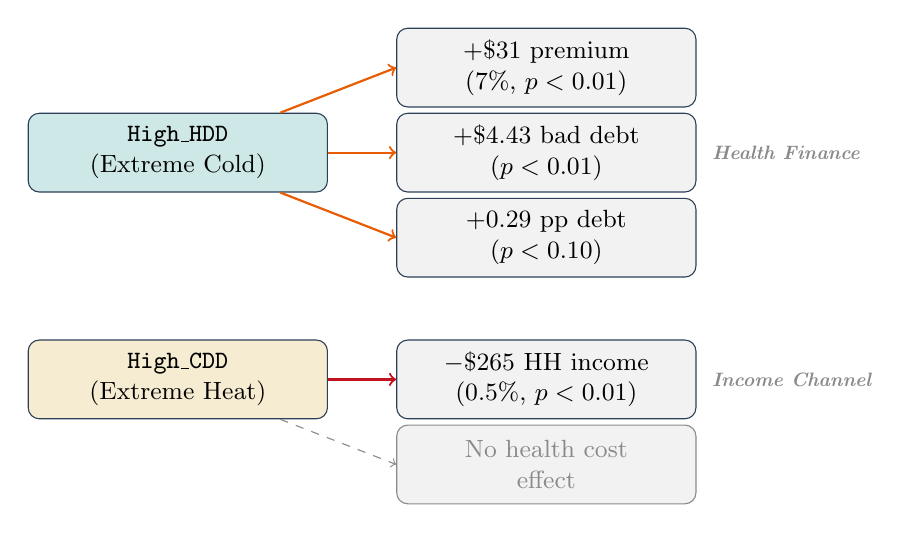
\begin{tikzpicture}[scale=0.9,
      box/.style={draw=DeepNavy, rounded corners=4pt, fill=LightGray,
                  minimum width=3.8cm, minimum height=1.0cm, align=center, font=\small}]
      % Causes
      \node[box, fill=Teal!20] (cold) at (0,0)    {\texttt{High\_HDD}\\(Extreme Cold)};
      \node[box, fill=Gold!20] (heat) at (0,-3.2) {\texttt{High\_CDD}\\(Extreme Heat)};
      % Outcomes
      \node[box] (prem) at (5.2, 1.2)  {$+\$31$ premium\\(7\%, $p<0.01$)};
      \node[box] (bad)  at (5.2, 0.0)  {$+\$4.43$ bad debt\\($p<0.01$)};
      \node[box] (debt) at (5.2,-1.2)  {$+0.29$ pp debt\\($p<0.10$)};
      \node[box] (inc)  at (5.2,-3.2)  {$-\$265$ HH income\\(0.5\%, $p<0.01$)};
      \node[box, draw=WarmGray, text=WarmGray] (none) at (5.2,-4.4) {No health cost\\effect};
      % Arrows — to .west for precise connection
      \draw[->, WarmOrange, thick] (cold) -- (prem.west);
      \draw[->, WarmOrange, thick] (cold) -- (bad.west);
      \draw[->, WarmOrange, thick] (cold) -- (debt.west);
      \draw[->, DeepRed,    thick] (heat) -- (inc.west);
      \draw[->, WarmGray, dashed]  (heat) -- (none.west);
      % Channel labels
      \node[font=\scriptsize\itshape\bfseries, text=WarmGray, anchor=west] at (7.4, 0.0)  {Health Finance};
      \node[font=\scriptsize\itshape\bfseries, text=WarmGray, anchor=west] at (7.4,-3.2) {Income Channel};
    \end{tikzpicture}
  \end{center}
  \vspace{0.2em}
  \begin{center}
    \tealtext{This asymmetry is a novel contribution to the climate-health literature}
  \end{center}
\end{frame}

% ══════════════════════════════════════════════════════════════════════════════
\transitionslide{Drought \& Air Quality}{Suggestive, Not Yet Causal}

% ── Drought ───────────────────────────────────────────────────────────────────
\begin{frame}{Drought: Suggestive Patterns, Pre-Trend Failure}
  \begin{columns}[T]
    \begin{column}{0.56\textwidth}
      \small
      \begin{tabular}{lrrl}
        \toprule
        Outcome & Est. & (SE) & \\
        \midrule
        Silver Premium & +\$18.3 & (14.1) & \graytext{n.s.} \\
        Medical Debt & --\$16 & (21) & \graytext{n.s.} \\
        Civilian Employed & --1,507 & (1,409) & \graytext{n.s.} \\
        \bottomrule
      \end{tabular}
      \vspace{0.5em}
      \begin{alertblock}{Pre-trend failure (DL)}
        $h=-2$ premium effect: +\$36 (p=0.0003)\\
        \graytext{\footnotesize Parallel trends violated; cannot claim causality}
      \end{alertblock}
    \end{column}
    \begin{column}{0.40\textwidth}
      \textbf{Why pre-trend failure?}\\[0.3em]
      Drought is rare (2.3\% of county-years) and concentrated in the Southwest. Pre-existing premium trends in drought-prone areas may reflect broader region-level policy or insurer responses.\\[0.5em]
      \tealtext{Interpretation: suggestive of a drought--premium link; future work needed to address selection}
    \end{column}
  \end{columns}
\end{frame}

% ── AQI ───────────────────────────────────────────────────────────────────────
\begin{frame}{Air Quality: Promising but Data-Sparse}
  \begin{columns}[T]
    \begin{column}{0.56\textwidth}
      \small
      \begin{tabular}{lrrl}
        \toprule
        Outcome & Est. & (SE) & $N$ \\
        \midrule
        Medical Debt Share & +0.05 pp & (0.09) & 11,143 \\
        Silver Premium & +\$5.9 & (4.1) & 8,942 \\
        Median HH Income & --\$51 & (53) & 11,155 \\
        \bottomrule
      \end{tabular}
      \vspace{0.5em}
      \begin{alertblock}{Data limitation}
        EPA ground monitors cover $\approx40\%$ of counties; sparse in early years. Sample is more urban, larger, higher-income.
      \end{alertblock}
    \end{column}
    \begin{column}{0.40\textwidth}
      \textbf{Future direction:}\\[0.3em]
      Replace sparse monitor data with NASA MODIS satellite PM$_{2.5}$ estimates (universal coverage)\\[0.5em]
      \tealtext{Lagged AQI effects ($h=2$) showed promise in county descriptives; not yet robust in event study}
    \end{column}
  \end{columns}
\end{frame}

% ══════════════════════════════════════════════════════════════════════════════
\transitionslide{Robustness}{DL vs.\ LP, Pre-Trends, Clustering}

% ── Dynamic Profiles Panel ────────────────────────────────────────────────────
\begin{frame}{Dynamic Profiles: All Significant Pairs}
  \begin{center}
    \includegraphics[width=0.88\textwidth]{../Analysis/plots/synthesis/synthesis_dynamic_profiles.png}
  \end{center}
  \graytext{\footnotesize LP impulse-response estimates across horizons $h=0$ to $h=3$ for all significant shock--outcome pairs (90\% CI)}
\end{frame}

% ── Robustness Panel ──────────────────────────────────────────────────────────
\begin{frame}{DL, LP, and Shock-History Controls All Agree}
  \begin{center}
    \includegraphics[width=0.88\textwidth]{../Analysis/plots/synthesis/synthesis_robustness_panel.png}
  \end{center}
  \graytext{\footnotesize Three estimators compared for premium and medical debt outcomes. Shaded = 90\% CI. LP+History adds prior-year shock controls.}
\end{frame}

% ── Pre-Trends Table ─────────────────────────────────────────────────────────
\begin{frame}{Pre-Trend Validity Summary}
  \begin{center}
    \small
    \begin{tabular}{llrll}
      \toprule
      \textbf{Shock} & \textbf{Outcome} & $\hat\beta_{h=-2}$ & $p$ & \textbf{Status} \\
      \midrule
      \texttt{High\_HDD} & Silver Premium & 9.2 & 0.52 & \tealtext{Pass} \\
      \texttt{High\_HDD} & Hosp.\ Bad Debt & 0.9 & 0.64 & \tealtext{Pass} \\
      \texttt{High\_CDD} & Median HH Income & --92.7 & 0.27 & \tealtext{Pass} \\
      \texttt{Any\_Shock} & Silver Premium & --1.3 & 0.62 & \tealtext{Pass} \\
      \midrule
      \texttt{Is\_Extreme\_Drought} & Silver Premium (DL) & +36.2 & 0.0003 & \emphcolor{Fail} \\
      \texttt{High\_AQI\_Max} & Silver Premium (DL) & +8.3 & 0.040 & \emphcolor{Fail} \\
      \texttt{High\_AQI\_Max} & Medical Debt (DL) & +0.003 & 0.0001 & \emphcolor{Fail} \\
      \bottomrule
    \end{tabular}
  \end{center}
  \vspace{0.3em}
  Cold and heat results pass. Drought and AQI premium effects do \emphcolor{not} satisfy parallel trends $\Rightarrow$ reported as suggestive only.
\end{frame}

% ── Multicollinearity ─────────────────────────────────────────────────────────
\begin{frame}{Multicollinearity: All VIFs Below 5.33}
  \begin{columns}[T]
    \begin{column}{0.48\textwidth}
      \small
      \begin{tabular}{lr}
        \toprule
        \textbf{Predictor} & \textbf{Max VIF} \\
        \midrule
        PDSI\_Lag1 & 4.96 \\
        PDSI\_Lag2 & 3.88 \\
        Z\_Temp\_Lag1 & 1.93 \\
        Z\_Precip\_Lag1 & 2.95 \\
        High\_HDD & 3.12 \\
        High\_CDD & 2.84 \\
        \bottomrule
      \end{tabular}
    \end{column}
    \begin{column}{0.48\textwidth}
      \begin{block}{Decision rule}
        VIF $< 5$: acceptable\\
        VIF $5$--$10$: moderate concern\\
        VIF $> 10$: severe\\[0.3em]
        \tealtext{All predictors below 5.33}\\[0.2em]
        \graytext{\footnotesize Pruned full 9-variable drought block (PDSI/PHDI/PMDI) to PDSI only for primary specs}
      \end{block}
    \end{column}
  \end{columns}
\end{frame}

% ══════════════════════════════════════════════════════════════════════════════
\transitionslide{Policy Implications}{What Should Policymakers Take Away?}

% ── Policy Slide ──────────────────────────────────────────────────────────────
\begin{frame}{Three Policy-Relevant Findings}
  \small
  \begin{block}{1. Cold-vulnerable regions carry higher insurance costs}
    Northern counties face \emphcolor{+7\% premiums} and \emphcolor{elevated hospital bad debt}.\\
    \tealtext{Policy lever:} Winterization investment; cold-weather risk pools; reinsurance corridors.
  \end{block}
  \vspace{0.2em}
  \begin{block}{2. Heat adaptation is working---but income is eroding}
    No health cost effect from heat, but households lose \emphcolor{$\approx$\$265/year}.\\
    \tealtext{Policy lever:} Heat-resilience income supports; cooling assistance (analogous to LIHEAP).
  \end{block}
  \vspace{0.2em}
  \begin{alertblock}{3. Compounding shocks amplify premium stress}
    Each additional simultaneous shock adds \emphcolor{+\$8} to annual premiums (exploratory; $p=0.015$).\\
    \tealtext{Future work:} Multi-peril climate risk pricing in ACA rating regulations.
  \end{alertblock}
\end{frame}

% ── Magnitudes in Context ─────────────────────────────────────────────────────
\begin{frame}{Economic Magnitudes in Context}
  \begin{center}
    \small
    \begin{tabular}{lll}
      \toprule
      \textbf{Finding} & \textbf{Magnitude} & \textbf{Benchmark} \\
      \midrule
      Cold $\rightarrow$ premium & +7\% per year & Tobacco surcharge: 5--15\% \\
      Cold $\rightarrow$ bad debt & +\$4.43/capita & $\sim$\$443k per 100k county \\
      Heat $\rightarrow$ HH income & --0.5\% per year & Small but recurring \\
      Compounding shocks & +\$8/shock/year & \graytext{Exploratory} \\
      \bottomrule
    \end{tabular}
  \end{center}
  \vspace{0.6em}
  \begin{columns}[T]
    \begin{column}{0.48\textwidth}
      These are \tealtext{average treatment effects} across all affected counties.\\
      Tail counties (severe, repeated shocks) likely face multiples of these magnitudes.
    \end{column}
    \begin{column}{0.48\textwidth}
      \begin{exampleblock}{Literature context}
        \footnotesize
        Gasparrini et al.\ (2017): Cold kills more than heat in most climates --- consistent with cold dominating health finance here.
      \end{exampleblock}
    \end{column}
  \end{columns}
\end{frame}

% ── Caveats ───────────────────────────────────────────────────────────────────
\begin{frame}{Caveats \& Limitations}
  \begin{columns}[T]
    \begin{column}{0.48\textwidth}
      \textbf{Identification}
      \begin{itemize}
        \item Parallel trends fail for drought/AQI
        \item SUTVA: shocks spatially correlated; insurance spans counties
        \item CDD/HDD are cumulative, not peak-event measures
      \end{itemize}
      \vspace{0.4em}
      \textbf{Data}
      \begin{itemize}
        \item Premium data: 26\% missing (pre-2014 gaps)
        \item AQI monitors: 60\% of county-years missing
        \item Hospital data: 23\% missing
      \end{itemize}
    \end{column}
    \begin{column}{0.48\textwidth}
      \textbf{External validity}
      \begin{itemize}
        \item Period: post-ACA only (2011--23)
        \item US-specific health finance system
        \item AQI sample skews urban
      \end{itemize}
      \vspace{0.4em}
      \textbf{Compound shocks}
      \begin{itemize}
        \item Only 2.2\% of obs with $\geq 2$ simultaneous shocks
        \item Dose-response significant but under-powered
      \end{itemize}
    \end{column}
  \end{columns}
\end{frame}

% ── Next Steps ────────────────────────────────────────────────────────────────
\begin{frame}{Remaining Work \& Next Steps}
  \begin{columns}[T]
    \begin{column}{0.48\textwidth}
      \textbf{Dissertation writing (in progress)}
      \begin{itemize}
        \item Methods section (2--3 pp)
        \item Results section (4--5 pp)
        \item Discussion: cold story, heat paradox, policy
        \item Figure polish for final submission
      \end{itemize}
    \end{column}
    \begin{column}{0.48\textwidth}
      \textbf{Future research directions}
      \begin{itemize}
        \item Heat--income mechanism (labour supply? energy costs?)
        \item Satellite PM$_{2.5}$ to resolve AQI sparsity
        \item Drought confounders: state ag-policy responses
        \item 2024--25 extension: subsidy contraction effects
      \end{itemize}
    \end{column}
  \end{columns}
  \vspace{0.6em}
  \begin{center}
    \tealtext{\large Thank you. Questions welcome.}
  \end{center}
\end{frame}

% ══════════════════════════════════════════════════════════════════════════════
% ── Appendix ──────────────────────────────────────────────────────────────────
\transitionslide{Appendix}{Additional Figures \& Tables}

\begin{frame}{Appendix A: Outcome Trends Over Time}
  \begin{center}
    \includegraphics[width=0.88\textwidth,height=0.78\textheight,keepaspectratio]{../Analysis/plots/descriptive/fig2_outcome_index_trends.png}
  \end{center}
\end{frame}

\begin{frame}{Appendix B: Distribution Shifts, Early vs.\ Late Period}
  \begin{center}
    \includegraphics[width=0.88\textwidth]{../Analysis/plots/descriptive/fig3_distribution_shift.png}
  \end{center}
\end{frame}

\begin{frame}{Appendix C: Cold $\rightarrow$ Medical Debt Share (LP)}
  \begin{center}
    \includegraphics[width=0.75\textwidth]{../Analysis/plots/event_study/lp_High_HDD_Medical_Debt_Share.png}
  \end{center}
\end{frame}

\begin{frame}{Appendix D: Robustness --- Extra Outcomes}
  \begin{center}
    \includegraphics[width=0.88\textwidth]{../Analysis/plots/synthesis/synthesis_robustness_panel_extra.png}
  \end{center}
\end{frame}

\begin{frame}{Appendix E: Full Contemporaneous Effects Table}
  \small
  \begin{center}
    \begin{tabular}{llrrl}
      \toprule
      \textbf{Shock} & \textbf{Outcome} & \textbf{Est.} & \textbf{(SE)} & $p$ \\
      \midrule
      Is\_Extreme\_Drought & Med.\ Debt Share     & --0.000 & (0.003) & 0.98 \\
      Is\_Extreme\_Drought & Silver Premium       & +18.3   & (14.1)  & 0.20 \\
      Is\_Extreme\_Drought & Hosp.\ Bad Debt/cap  & +1.3    & (3.3)   & 0.69 \\
      High\_CDD & Med.\ Debt Share               & --0.003 & (0.003) & 0.29 \\
      High\_CDD & Silver Premium                 & --2.4   & (10.0)  & 0.82 \\
      High\_CDD & Median HH Income               & --\$265 & (87)    & 0.004 \\
      High\_HDD & Med.\ Debt Share               & +0.003  & (0.002) & 0.06 \\
      High\_HDD & Silver Premium                 & +\$30.7 & (9.9)   & 0.003 \\
      High\_HDD & Hosp.\ Bad Debt/cap            & +\$4.4  & (1.6)   & 0.008 \\
      High\_AQI\_Max & Med.\ Debt Share          & +0.001  & (0.001) & 0.64 \\
      High\_AQI\_Max & Silver Premium            & +\$5.9  & (4.1)   & 0.15 \\
      Any\_Shock & Silver Premium                & +\$8.5  & (4.6)   & 0.07 \\
      \bottomrule
    \end{tabular}
  \end{center}
  \graytext{\footnotesize LP, $h=0$, unweighted, state-clustered. * $p<0.10$, ** $p<0.05$, *** $p<0.01$}
\end{frame}

\end{document}
